%% ma: L12-B01-0021
%% lop: 12
%% chuong: 1
%% bai: 1
%% dang: 12.1.3
%% loai: TN4
%% muc: NB
%% dap_an: "D"
%% nguon: "(NBV)-ĐỀ SỐ 12-MỖI NGÀY 1 ĐỀ THI 2025.pdf (D12, MỖI NGÀY 1 ĐỀ - Đề số 12), Phần I Câu 1"
%% kien_thuc: "Bài 1 (dấu của đạo hàm và tính đơn điệu)"
%% trang_thai: chinh-thuc
%% ghi_chu: "Đáp án gốc D đúng. Bảng xét dấu dựng lại bằng tkz-tab từ hình gốc."
\begin{ex}
Cho hàm số $y=f(x)$ có bảng xét dấu của đạo hàm như sau:
\begin{center}
\begin{tikzpicture}
  \tkzTabInit[lgt=1.4,espcl=2.6]{$x$/.8,$f'(x)$/.8}{$-\infty$,$-4$,$-2$,$0$,$+\infty$}
  \tkzTabLine{,-,0,+,0,-,0,+,}
\end{tikzpicture}
\end{center}
Khẳng định nào sau đây đúng?
\choice{Hàm số đã cho đồng biến trên khoảng $(-\infty;-4)$}{Hàm số đã cho đồng biến trên khoảng $(-2;0)$}{Hàm số đã cho đồng biến trên khoảng $(-\infty;-2)$}{\True Hàm số đã cho đồng biến trên khoảng $(0;+\infty)$}
\loigiai{Từ bảng xét dấu, $f'(x)>0$ trên $(-4;-2)$ và $(0;+\infty)$ nên hàm số đồng biến trên mỗi khoảng này; $f'(x)<0$ trên $(-\infty;-4)$ và $(-2;0)$ nên hàm số nghịch biến trên mỗi khoảng đó.

Khoảng $(0;+\infty)$ nằm trọn trong khoảng đồng biến. Các khoảng ở A, B nghịch biến, khoảng ở C chứa cả khoảng đồng biến lẫn nghịch biến. Chọn D.}
\end{ex}
